% !TeX root = ../Thesis.tex

%************************************************
\chapter{Implementation}\label{ch:implementation}
%************************************************
\glsresetall % Resets all acronyms to not used

In this chapter, we want to discuss the details of our implementation of text-based steganography on Android. First we will give a high-level overview of the app in \cref{sec:overviewOfTheApp}. Then \cref{sec:jni} will show an example of how Java/Kotlin and C++ code can interact using the \gls{JNI}. \cref{sec:tokenGenerationWithLlamaCpp} will introduce all necessary abstractions to understand token generation with llama.cpp. \cref{sec:algorithms} will explain the algorithms we used for steganography. So far, this is what was needed to port the functionality of Stegasuras~\cite{zieglerNeuralLinguisticSteganography2019} to Android.

We expand this functionality already in \cref{sec:algorithms} by implementing another compression algorithm. Then we will show how to improve cover text quality in \cref{sec:finishingTheLastSentence,sec:creatingAConversationBetweenCoverTexts,sec:emojis}: First we will show how to handle the last sentence, then how to create a conversation, and lastly how to generate emojis.

\section{Overview of the app}
\label{sec:overviewOfTheApp}
In this section, we will give a high-level overview of the app. We walk through every screen of the \gls{UI} and explain what functionality is offered and how to use it.

\subsection{Home screen}
\label{sec:homeScreen}
\cref{fig:homeScreen} shows the home screen of our app. The \gls{UI} is based on the Stegasuras demo~\cite{zieglerStegasuras2025}: We have two text input fields, a mode selector for encode/decode, a switch to toggle conversation on/off, and a start button. Furthermore, we have icons in the top corners for navigation to the other screens (see \cref{sec:conversationScreen,sec:settingsScreen}).

\begin{figure}
	\begin{wide}
		\captionsetup{width=\linewidth}
		\begin{subfigure}{0.45\linewidth}
			\centering
			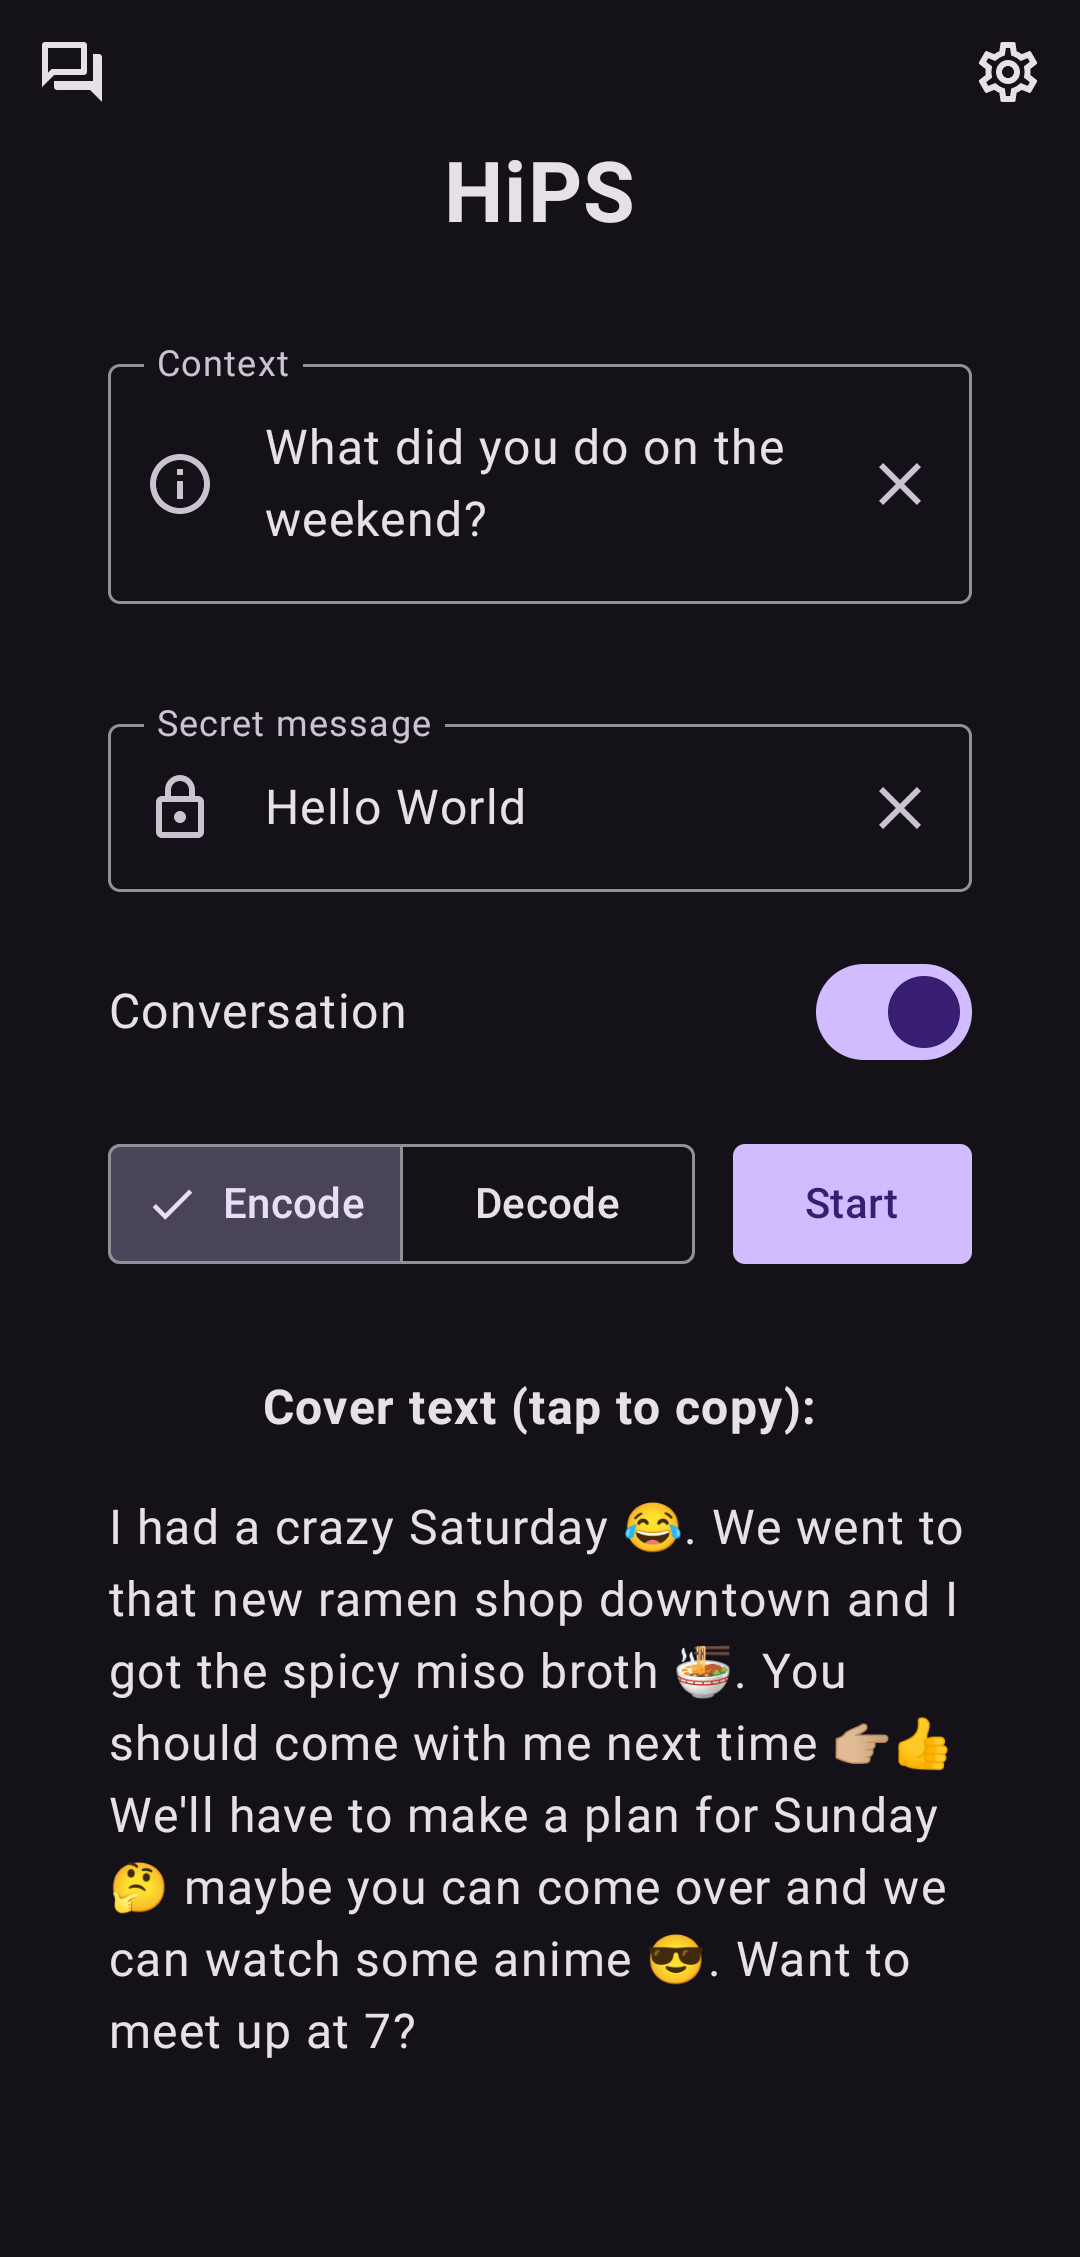
\includegraphics[width=\linewidth]{hips_home_screen_a.png}
			\caption{Encoding of a secret message.}
			\label{fig:homeScreenA}
		\end{subfigure}
        \hfill
		\begin{subfigure}{0.45\linewidth}
			\centering
			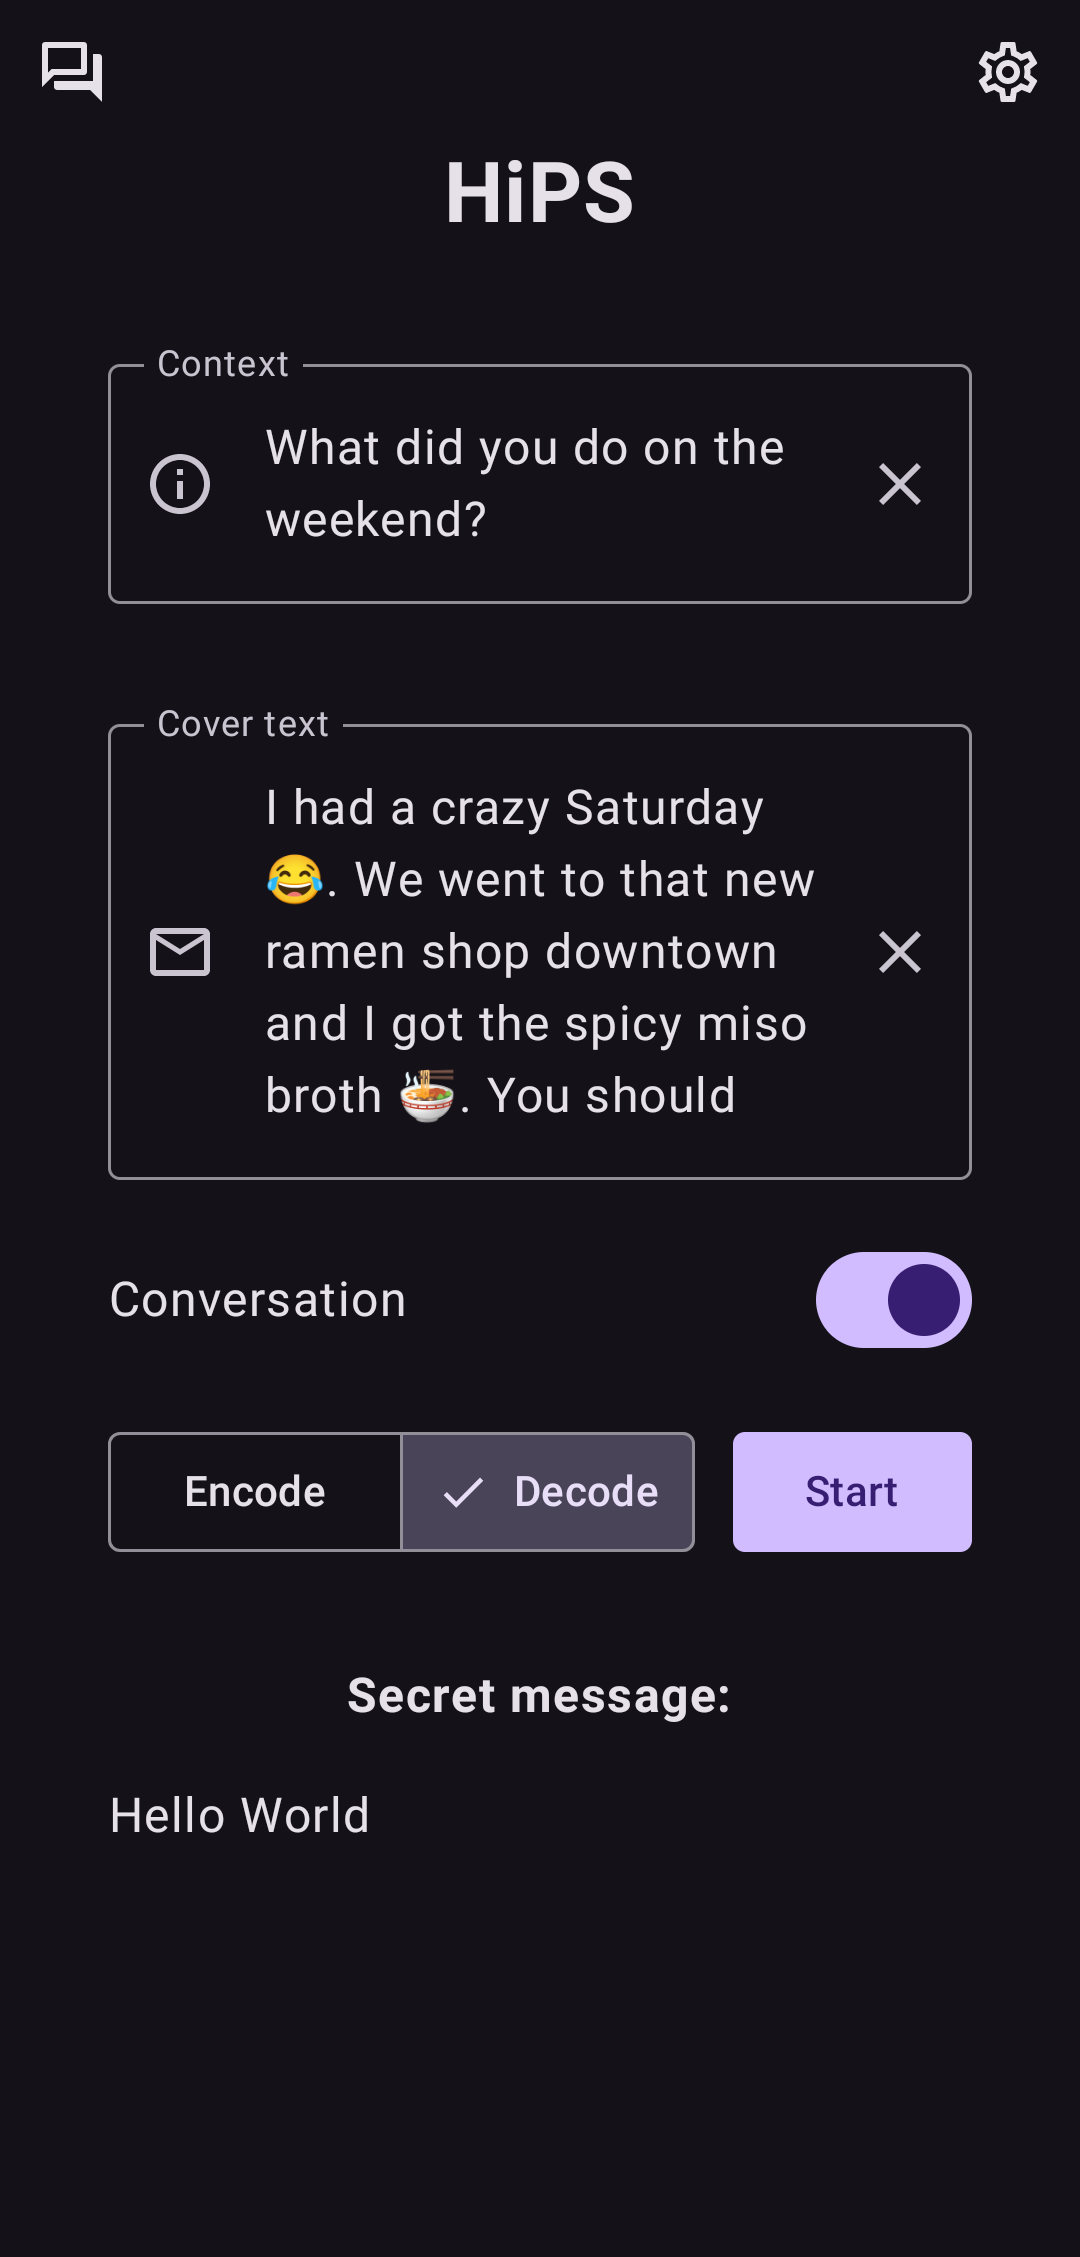
\includegraphics[width=\linewidth]{hips_home_screen_b.png}
			\caption{Decoding of a cover text.}
			\label{fig:homeScreenB}
		\end{subfigure}
		\caption[HiPS: Home screen]{Standalone functionality of HiPS on the home screen.}
		\label{fig:homeScreen}
	\end{wide}
\end{figure}

In encode mode, the text input fields are for the context to generate a cover text from, and for the secret message to be encoded in the cover text. After pressing the start button, the cover text will be generated and displayed at the bottom. Tapping it copies it to the clipboard. In decode mode, the text input fields are for the context the cover text. After pressing the start button, the secret message will be display at the bottom.

The functionality of Stegasuras is replicated by toggling the conversation switch off. The cover text is then generated by \textit{completing} the context. This opens up adjacent use cases, e.g. using a press statement to transfer information out of an organization.

When the conversation switch is toggled on, the functionality of Stegasuras is extended. The cover text is then generated by \textit{replying} to the context, i.e. the context is assumed to be a chat message. This uses the settings configurable on the settings screen (see \cref{sec:settingsScreen}). This standalone functionality helps users protect their privacy with existing instant messengers by simply copy-pasting messages.

\subsection{Conversation screen}
\label{sec:conversationScreen}
\cref{fig:conversationScreen} shows the conversation screen. This is a demo of how our steganography could be integrated into an instant messenger.

\begin{figure}
	\begin{wide}
		\captionsetup{width=\linewidth}
		\begin{subfigure}{0.45\linewidth}
			\centering
			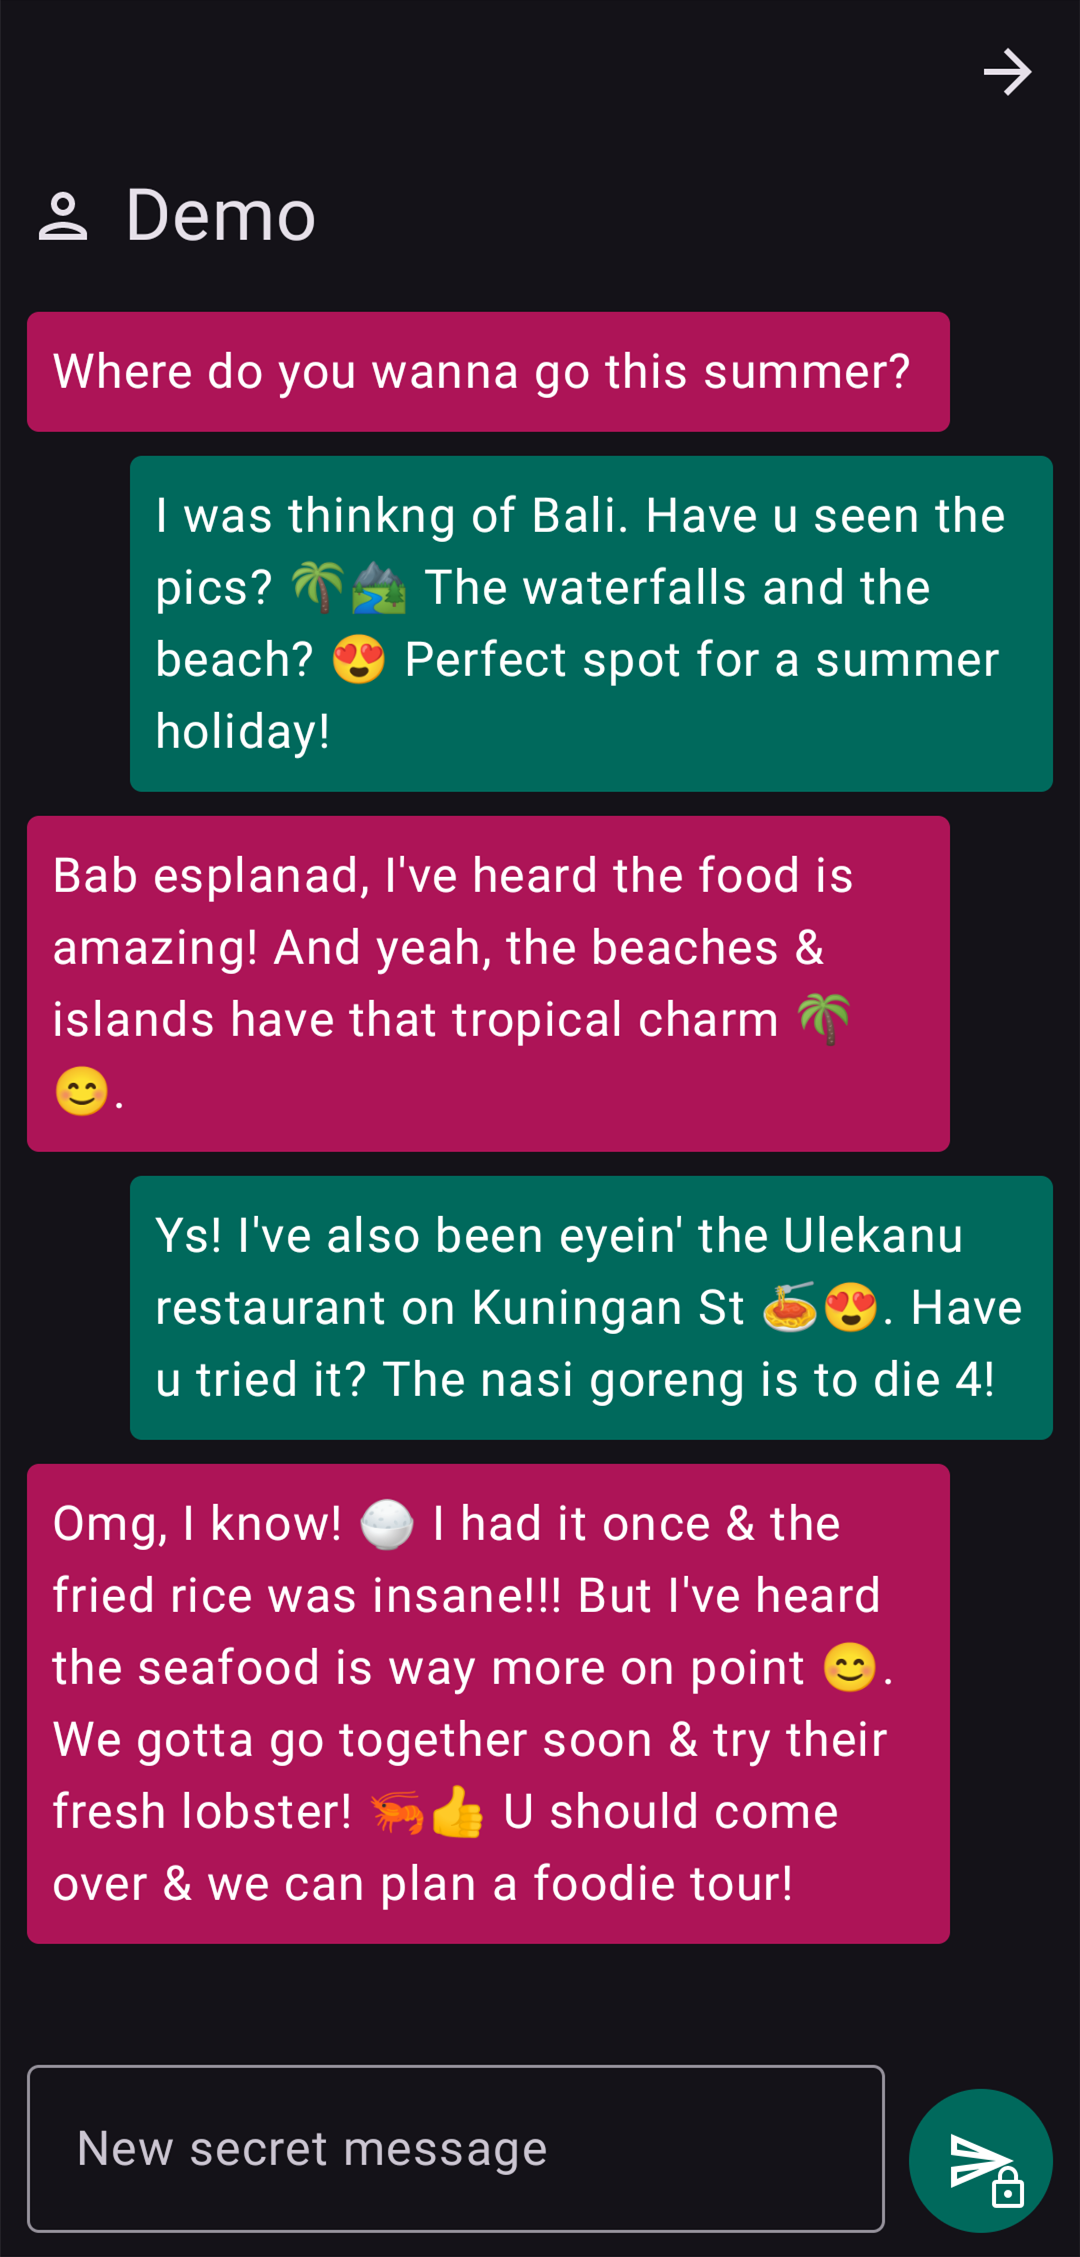
\includegraphics[width=\linewidth]{hips_conversation_screen_a.png}
			\caption{A conversation of cover texts.}
			\label{fig:conversationScreenA}
		\end{subfigure}
        \hfill
		\begin{subfigure}{0.45\linewidth}
			\centering
			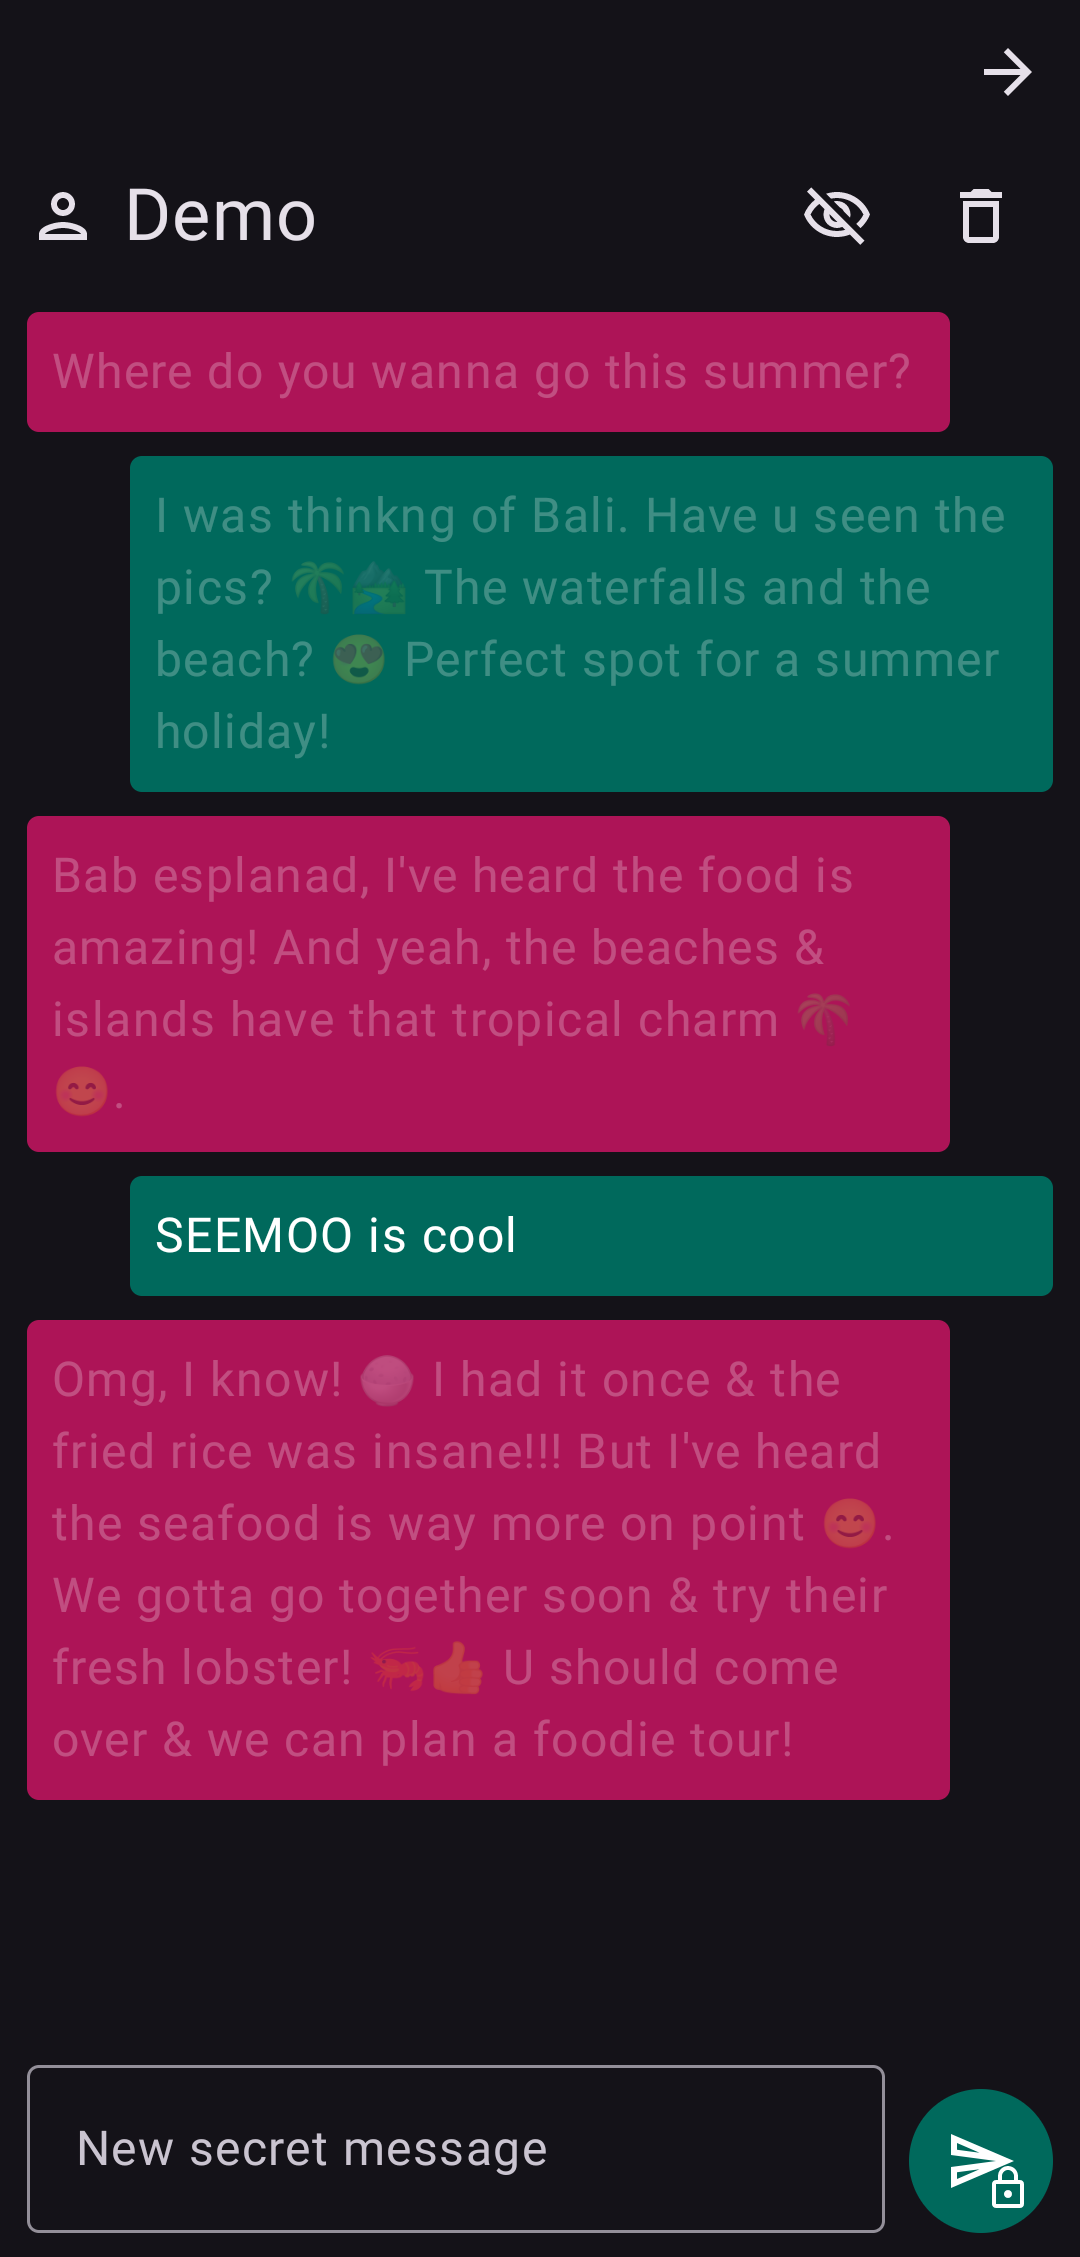
\includegraphics[width=\linewidth]{hips_conversation_screen_b.png}
			\caption{Showing a secret message.}
			\label{fig:conversationScreenB}
		\end{subfigure}
		\caption[HiPS: Conversation screen]{Steganography on the conversation screen.}
		\label{fig:conversationScreen}
	\end{wide}
\end{figure}

This screen displays a list of messages, a text input field and a send button. The messages are arranged as a chat conversation between two people and coloured correspondingly. The text input field allows the user to type in a new message, which then can be sent into the chat by pressing the send button. As this is a demo, they are not sent over the internet, but only stored locally. Effectively, the users chat with themselves by constantly switching roles. At the top, we have placeholders for name and profile picture of the chat partner, and a back button to navigate back to the home screen.

The send button can be long-pressed to toggle steganography on/off. The current mode is indicated by a lock being shown or hidden inside it. If steganography is toggled on, the message in the text input field is assumed to be a secret message and will be encoded into a cover text. The cover text is then sent into the conversation. Again, this can be configured on the settings screen (see \cref{sec:settingsScreen}): The system prompt and a number of prior messages are used as context to generate the cover text from. This corresponds to the conversation switch on the home screen being toggled on (see \cref{sec:homeScreen}). If steganography is toggled off, the message in the text input field is assumed to be a plain text message and will be sent as is. This allows for arbitrary plain text messages in-between cover texts.

When the text input field is blank, the send button can be short-pressed to switch roles. The current role is indicated by the send button being the same colour as the corresponding messages. This allows for sending multiple consecutive messages from the same role, i.e. roles to not be strictly alternating. The role also switches automatically after sending a message. Messages in the chat can also be long-pressed, which highlights them as being selected. Short-pressing unselects them again. If at least one message is selected, two new buttons will be displayed at the top: Decode and delete.

The decode button can only be pressed if exactly one message is currently selected. Otherwise, a toast is displayed to guide the user. This is to avoid running multiple instances of the \gls{LLM} simultaneously. Otherwise, the app process could be terminated by the Android operating system for excessive resource usage. When the decode button is pressed, it tries to decode the selected message. If decoding was successful (i.e. if the selected message was a cover text and not a plain text), the secret message will be displayed in place of the cover text. The symbol of the decode button changes to indicate that a secret message is visible. By pressing it again, the secret message and the two buttons are hidden again.

The delete button can only be pressed if the selected messages are at the end of the conversation. Otherwise, a toast is displayed again. This is to avoid corrupting the context for decoding a message by deleting messages prior to it. When the delete button is pressed, the selected messages will be deleted and the two buttons will be hidden again.

\subsection{Settings screen}
\label{sec:settingsScreen}
\cref{fig:settingsScreen} shows the settings screen. This is where the \gls{LLM} is managed and where all parameters of our algorithms can be modified. Upon installation of our app, the user needs to download the \gls{LLM} by pressing the download button at the top of this screen. Then the \gls{LLM} can be loaded into or unloaded from memory by pressing the start/stop button below the download button. Pressing this button is only necessary after downloading the \gls{LLM} when using our app for the first time. Afterwards, the \gls{LLM} is automatically loaded on startup.

\begin{figure}
	\begin{wide}
		\captionsetup{width=\linewidth}
		\begin{subfigure}{0.3\linewidth}
			\centering
			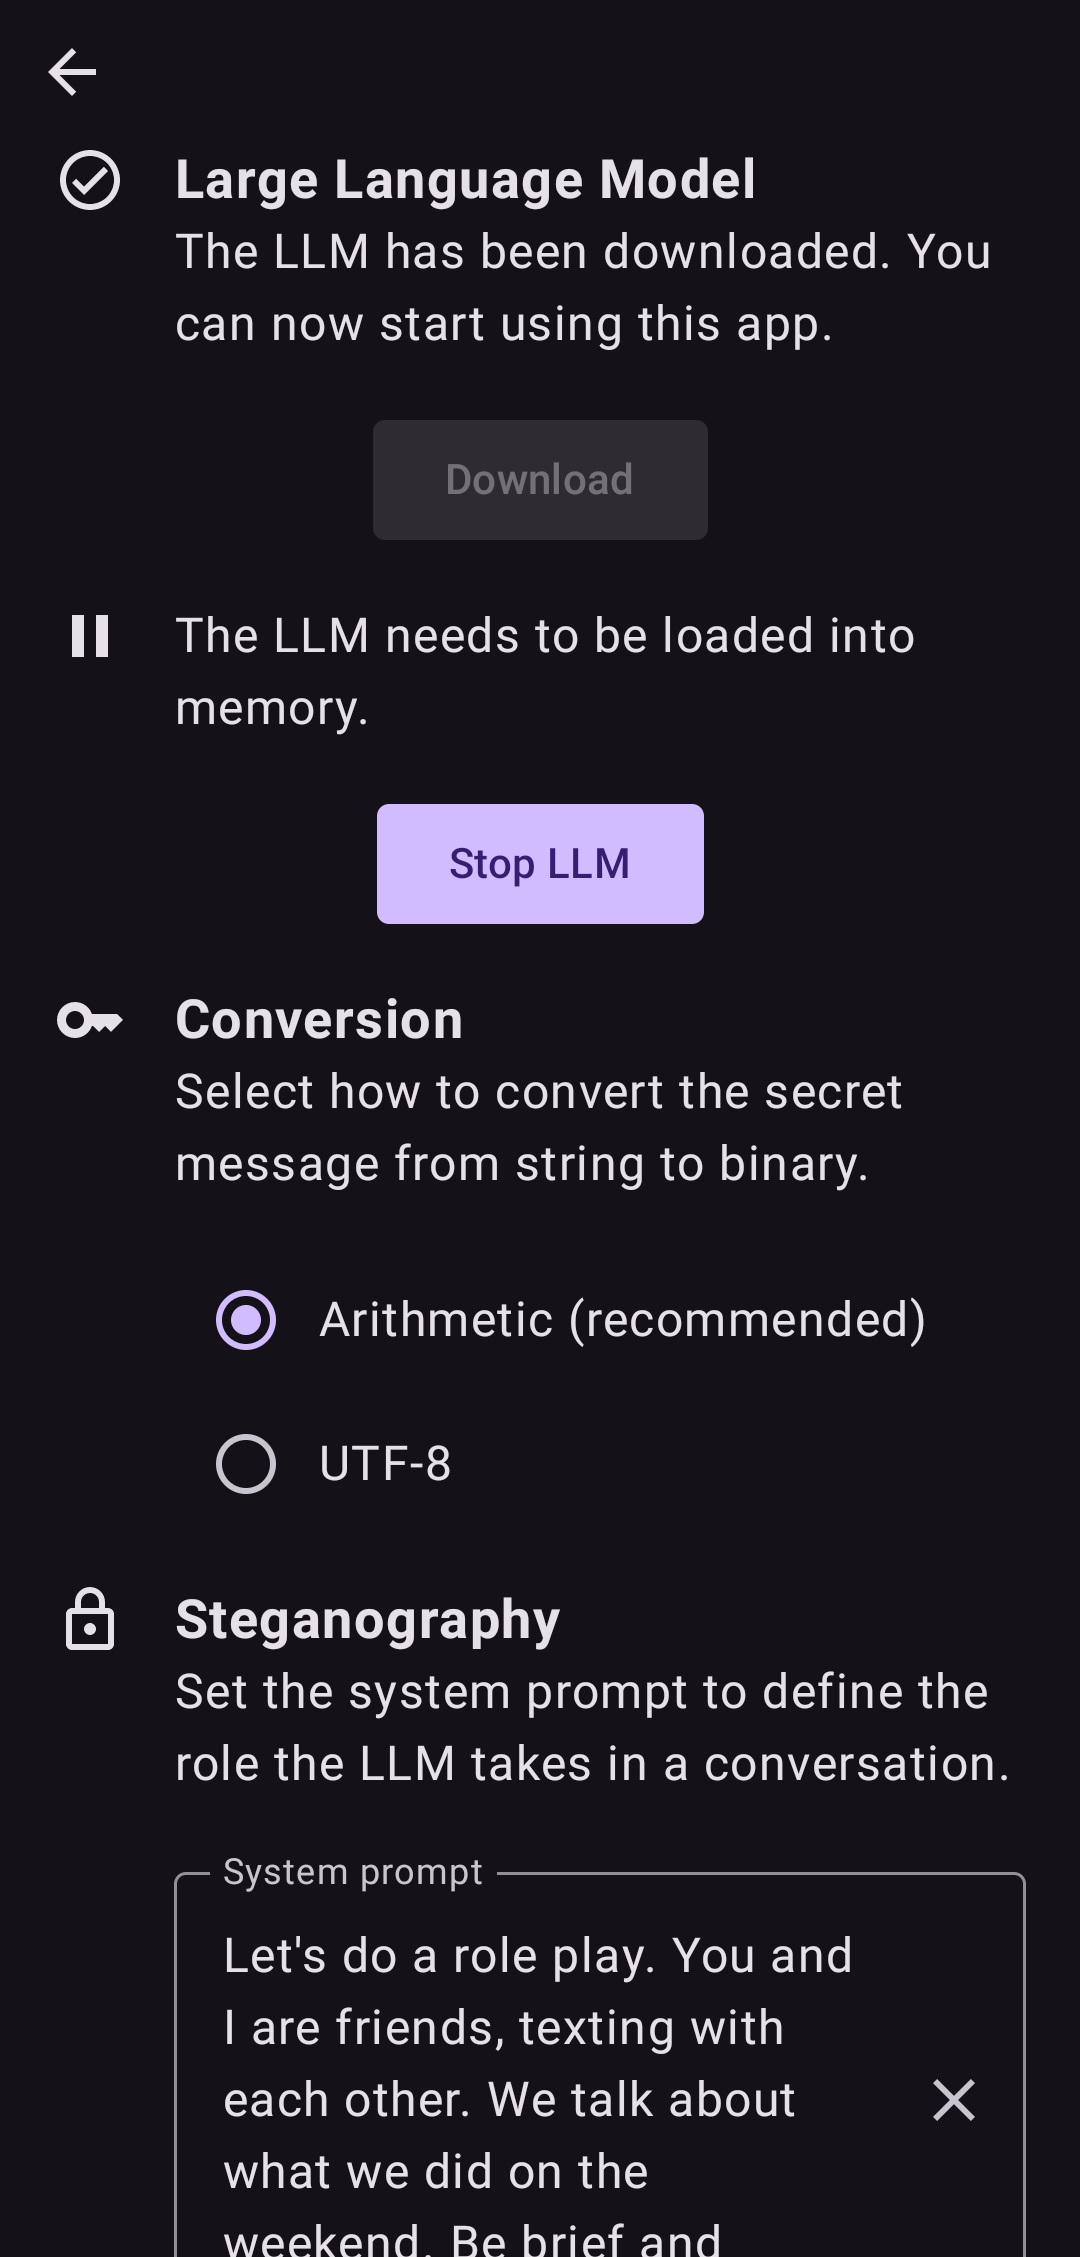
\includegraphics[width=\linewidth]{hips_settings_screen_a.png}
			\caption{Download button, start button and binary conversion mode.}
			\label{fig:settingsScreenA}
		\end{subfigure}
        \hfill
        \begin{subfigure}{0.3\linewidth}
			\centering
			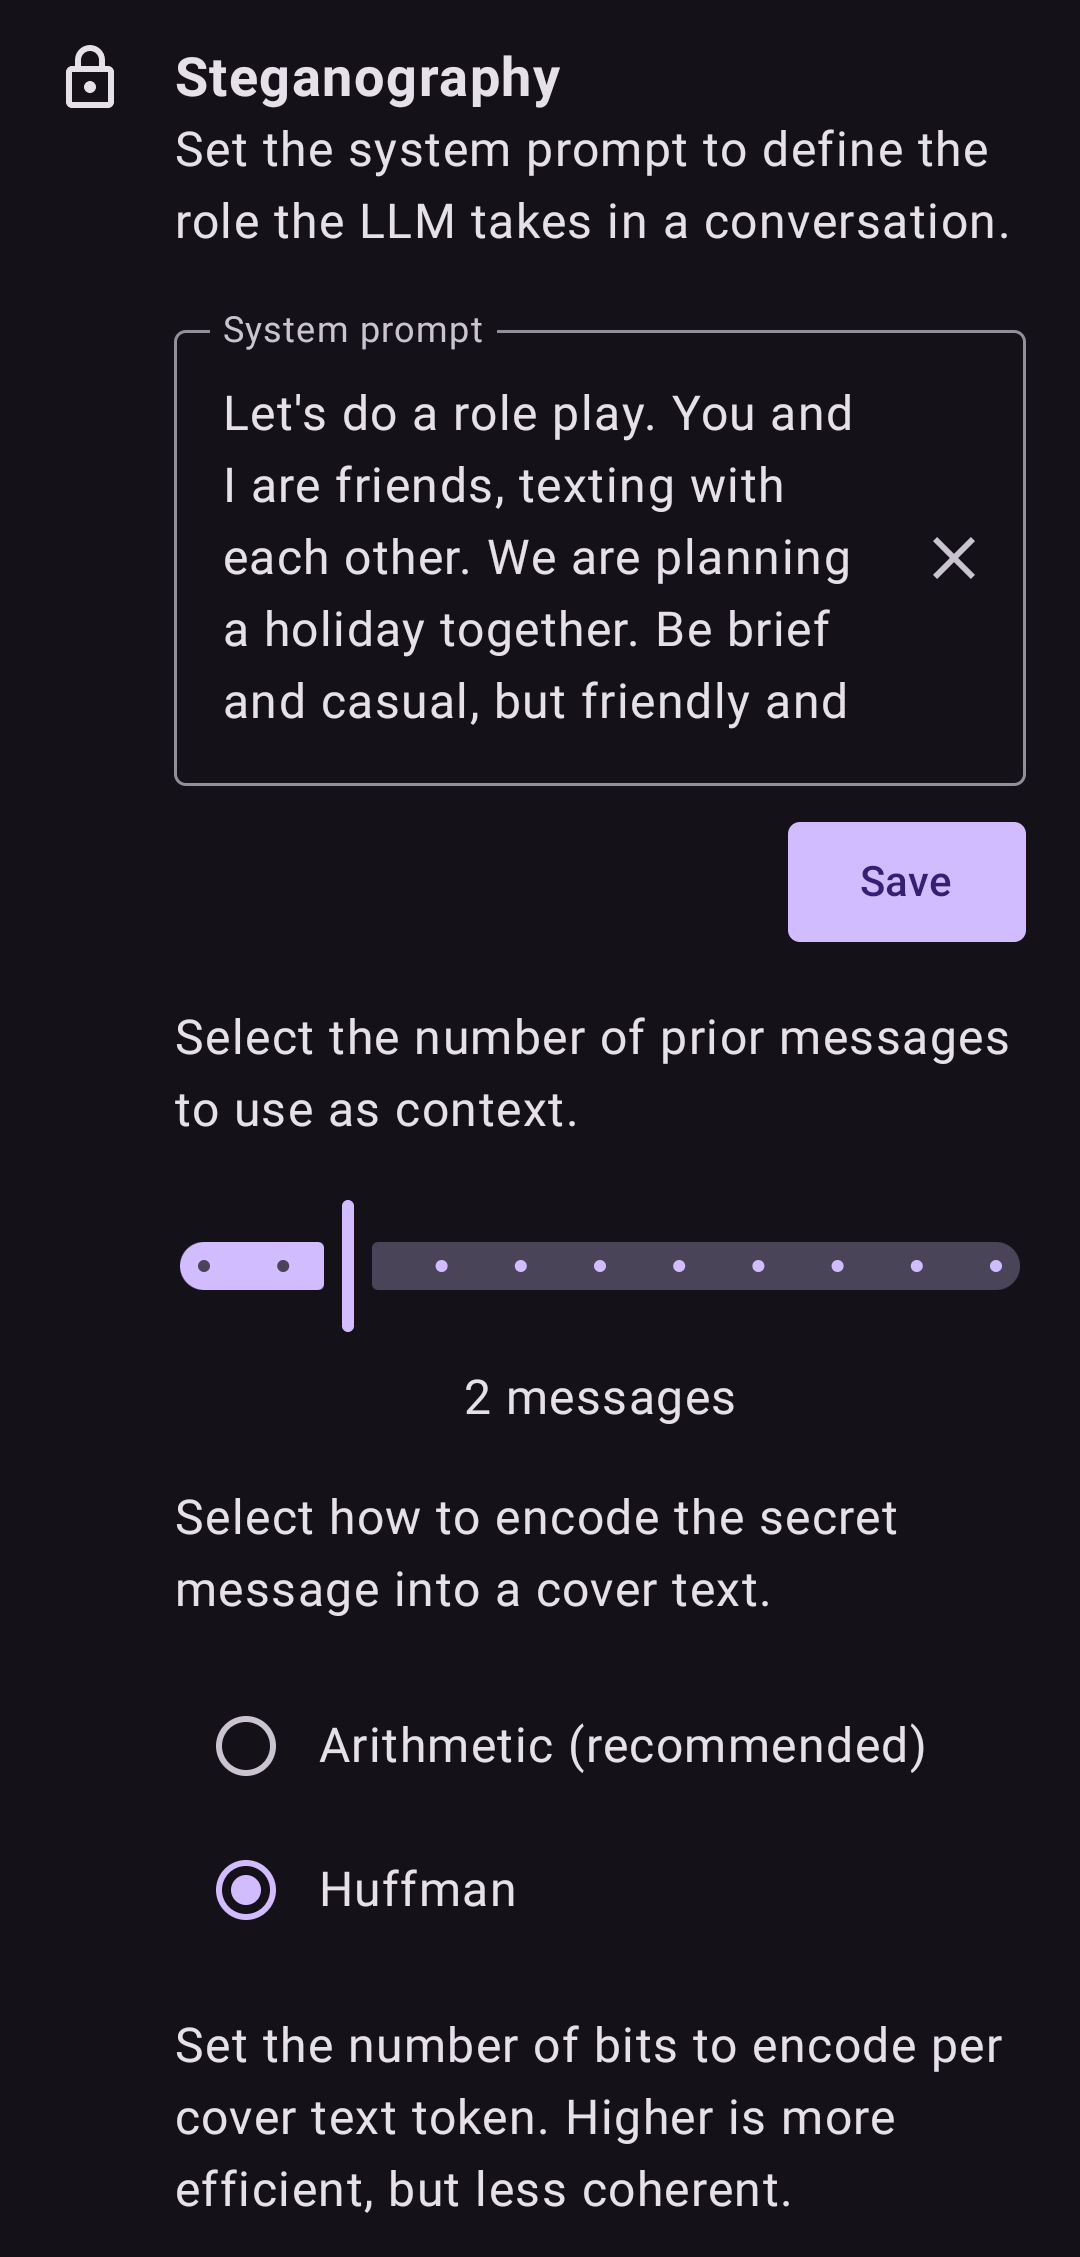
\includegraphics[width=\linewidth]{hips_settings_screen_b.png}
			\caption{System prompt, context length and steganography mode.}
			\label{fig:settingsScreenB}
		\end{subfigure}
        \hfill
        \begin{subfigure}{0.3\linewidth}
			\centering
			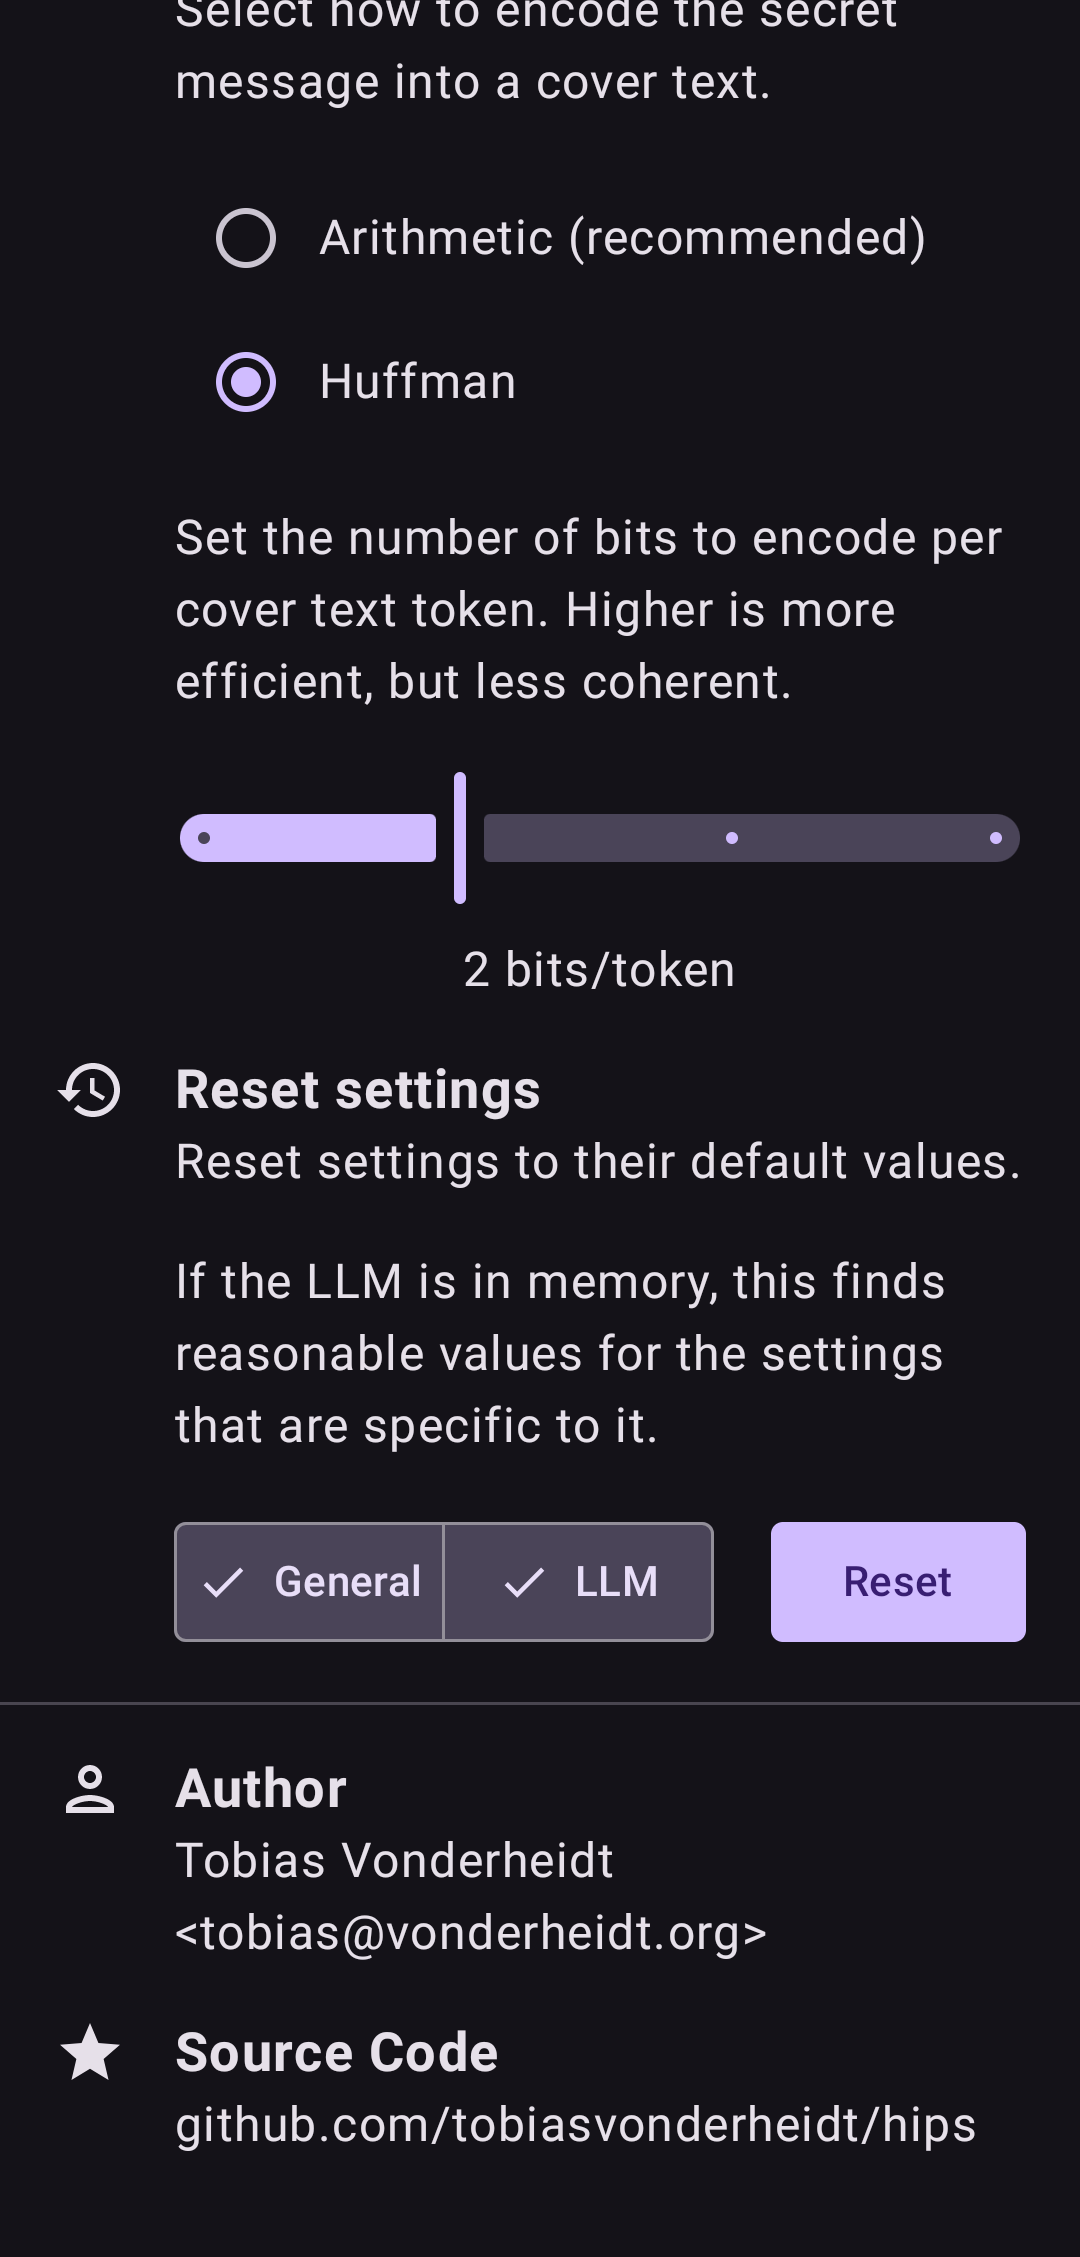
\includegraphics[width=\linewidth]{hips_settings_screen_c.png}
			\caption{Algorithm-specific settings for Huffman coding and reset options.}
			\label{fig:settingsScreenC}
		\end{subfigure}
		\caption[HiPS: Conversation screen]{The settings screen.}
		\label{fig:settingsScreen}
	\end{wide}
\end{figure}

Below these buttons, there are various selectors, sliders and input fields for the parameters of our algorithms. They are arranged in the order of corresponding steps during the encoding process. First there is a selector for the conversion mode, i.e. for how to convert the secret message from string to binary. It offers \lstinline|Arithmetic (recommended)|, \lstinline|Huffman| and \lstinline|UTF-8| as options. \lstinline|UTF-8| serves as a baseline as it doesn't compress the secret message, while \lstinline|Arithmetic| compresses it using the \gls{LLM} and \lstinline|Huffman| compresses it without using the \gls{LLM}. This will be explained in detail in \cref{sec:binaryConversionAndCompression}.

This is followed by a text input field for a system prompt. This is a natural language command that can be passed to the \gls{LLM} to influence its behaviour. This is relevant for the conversation screen, and for the home screen if the conversation switch there is toggled on. A more detailed explanation for how the system prompt is used will be given in \cref{sec:creatingAConversationBetweenCoverTexts}.

Afterwards, there is a slider to select a number of messages between 0 and 10. This is the number of prior messages to be used as context on the conversation screen. It is not relevant for the home screen, as context length is always fixed to 1 message there. While values 1 to 10 be used as is, 0 is interpreted as \lstinline|All messages|. This means, all prior messages will be used as context to generate the next cover text from. It is recommended to set this to a value in the 1-10 range to limit resource usage when a conversation contains many messages.

Furthermore, we have a selector for the steganography algorithm. It offers \lstinline|Arithmetic (recommended)| and \lstinline|Huffman| as options. Depending on the selected algorithm, its specific parameters can be set below this selector (see \cref{sec:steganographyEncodingDecoding} for details).

When \lstinline|Arithmetic| is selected, there are sliders for the \lstinline|temperature|, \lstinline|topK| and \lstinline|precision| parameters. The \lstinline|temperature| slider ranges from 0.0 to 2.0 in steps of 0.1, but can't be 0.0 as we will need to divide by the \lstinline|temperature| value. The \lstinline|topK| slider ranges from 0 to 100\% of the vocabulary size of the \gls{LLM}. The \lstinline|precision| slider ranges from 0 to 32 bits. Both \lstinline|topK| and \lstinline|precision| are only visible when the \gls{LLM} is in memory, as the vocabulary size for \lstinline|topK| is specific to each \gls{LLM} and the recommended value for \lstinline|precision| depends on it.

When \lstinline|Huffman| is selected, there is a slider for the \lstinline|bitsPerToken| parameter. It determines the height of the Huffman tree and therefore the bits encoded in every cover text token. The slider ranges from 0 to 4.

Lastly, there is a button to reset all settings to their default values. It comes with a selector for whether to reset either only general settings, only settings that are specific to the \gls{LLM} (i.e. \lstinline|topK| and \lstinline|precision|), or both. When the \gls{LLM} is in memory, settings specific to it will be reset to sensible defaults. Otherwise, they are reset to 0.

\section{Java Native Interface}
\label{sec:jni}

\section{Token generation with llama.cpp}
\label{sec:tokenGenerationWithLlamaCpp}

\section{Algorithms}
\label{sec:algorithms}

\subsection{Binary conversion and compression}
\label{sec:binaryConversionAndCompression}

\subsubsection{Arithmetic compression}
\label{sec:arithmeticCompression}

\subsubsection{Huffman compression}
\label{sec:huffmanCompression}

\subsubsection{UTF-8}
\label{sec:utf8}

\subsection{Steganography encoding/decoding}
\label{sec:steganographyEncodingDecoding}

\subsubsection{Arithmetic coding}
\label{sec:arithmeticCoding}

\subsubsection{Huffman coding}
\label{sec:huffmanCoding}

\section{Finishing the last sentence}
\label{sec:finishingTheLastSentence}

\section{Creating a conversation between cover texts}
\label{sec:creatingAConversationBetweenCoverTexts}

\section{Emojis}
\label{sec:emojis}
